\section{Metodi: caratterizzare l'alveo}
Si è quantificato l'areale delle isole presenti in alveo avendo accortezza di distinguerlo chiaramente dall'areale della \emph{floodplain}, il quale è soggetto a dinamiche diverse rispetto alle isole.
\\
Per classificare il terreno occupato dall'alveo è stato seguito l'approccio di altri autori in analisi simili eseguite su immagini \AST{} e LandSat~TM \squarecites{Bertoldi:2011-ASTER}{Henshaw:2013-LandSat}.
\\
Sono stati ottenuti in seguito la larghezza media dell'alveo e la potenza della corrente di ogni tratto.

\subsection{Classificazione dell'alveo}
\paragraph{Maschera computazionale}
Dapprima è stata individuata manualmente una maschera di calcolo che comprendesse l'alveo attivo e la parte di piana alluvionale che è stata erosa quando coinvolta nelle piene; 
tale maschera si estende da Tolmezzo al ponte di Madrisio
(\cref{fig:esempio-maschera}). 
Applicandola, il dominio computazionale è stato ridotto, in modo tale da comprendere l'inviluppo degli alvei attivi che si sono succeduti dall'immagine del~2000 a quella del~2018.
%
\begin{figure}[t]
	\centering
	\begin{subfigure}[b]{0.4\textwidth}
		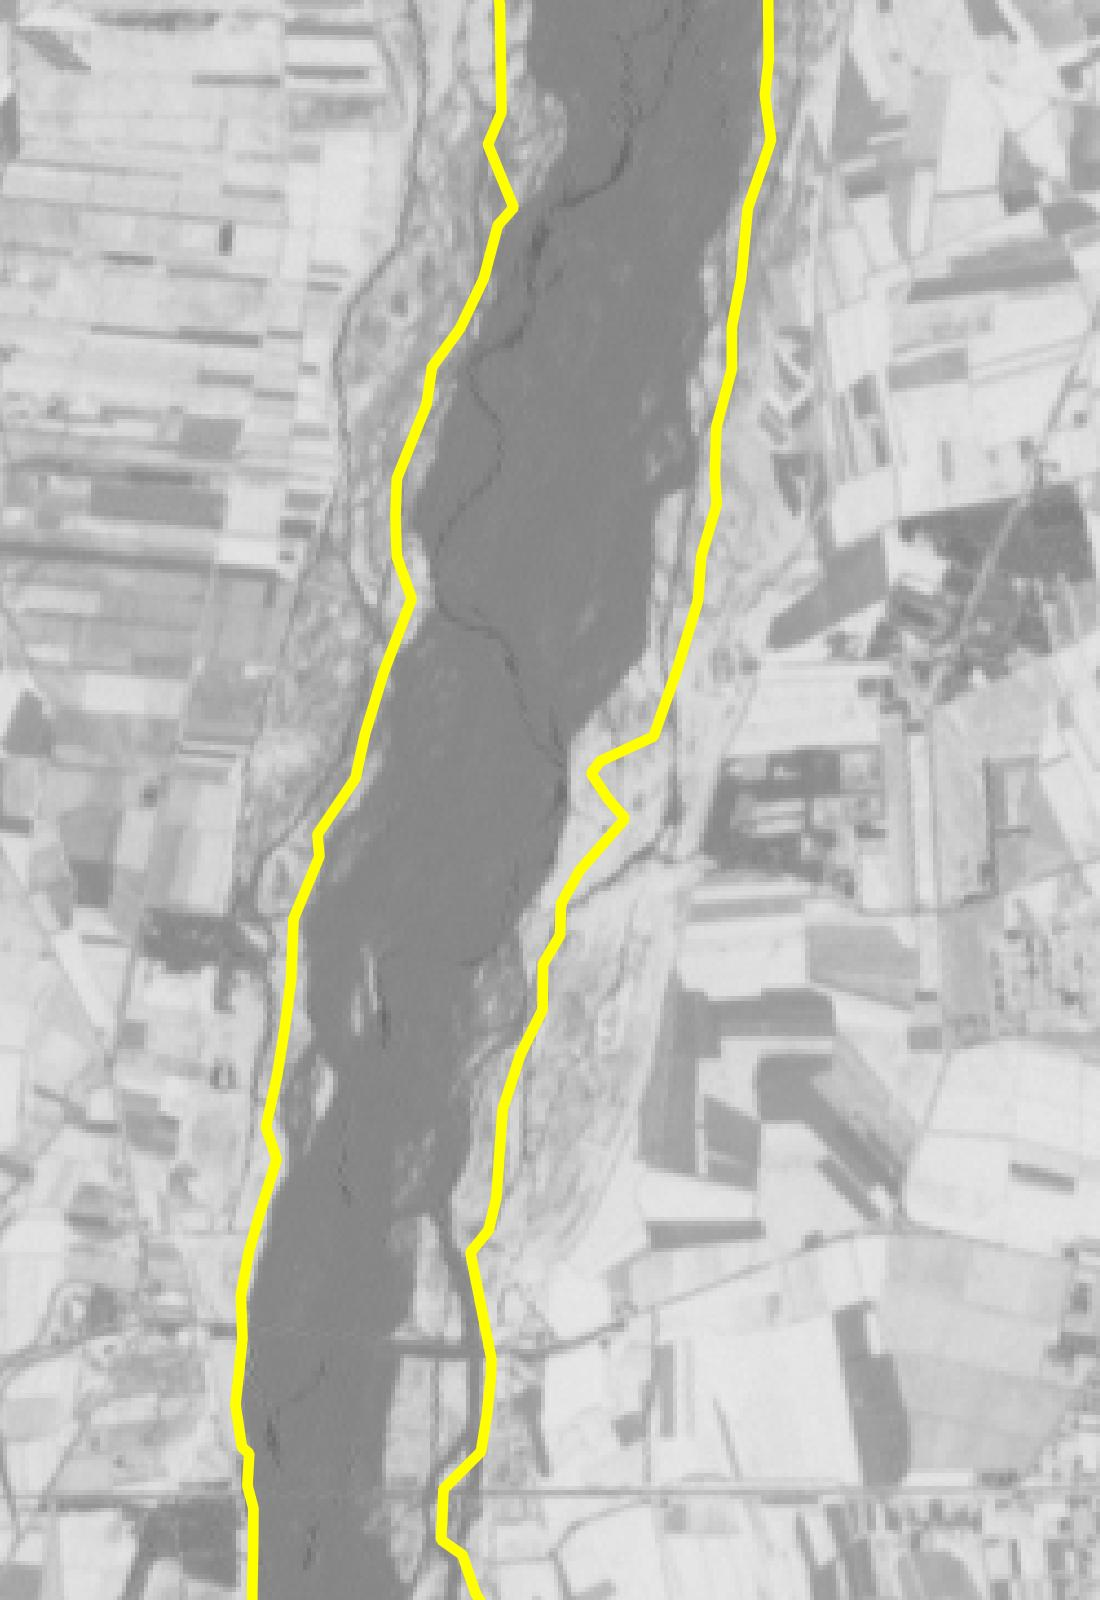
\includegraphics[width=\textwidth]{files/esempio_mask_2002_06_12.jpeg}
		\caption{\AST{} 2002-06-12.}
	\end{subfigure}
	\qquad
	\begin{subfigure}[b]{0.4\textwidth}
		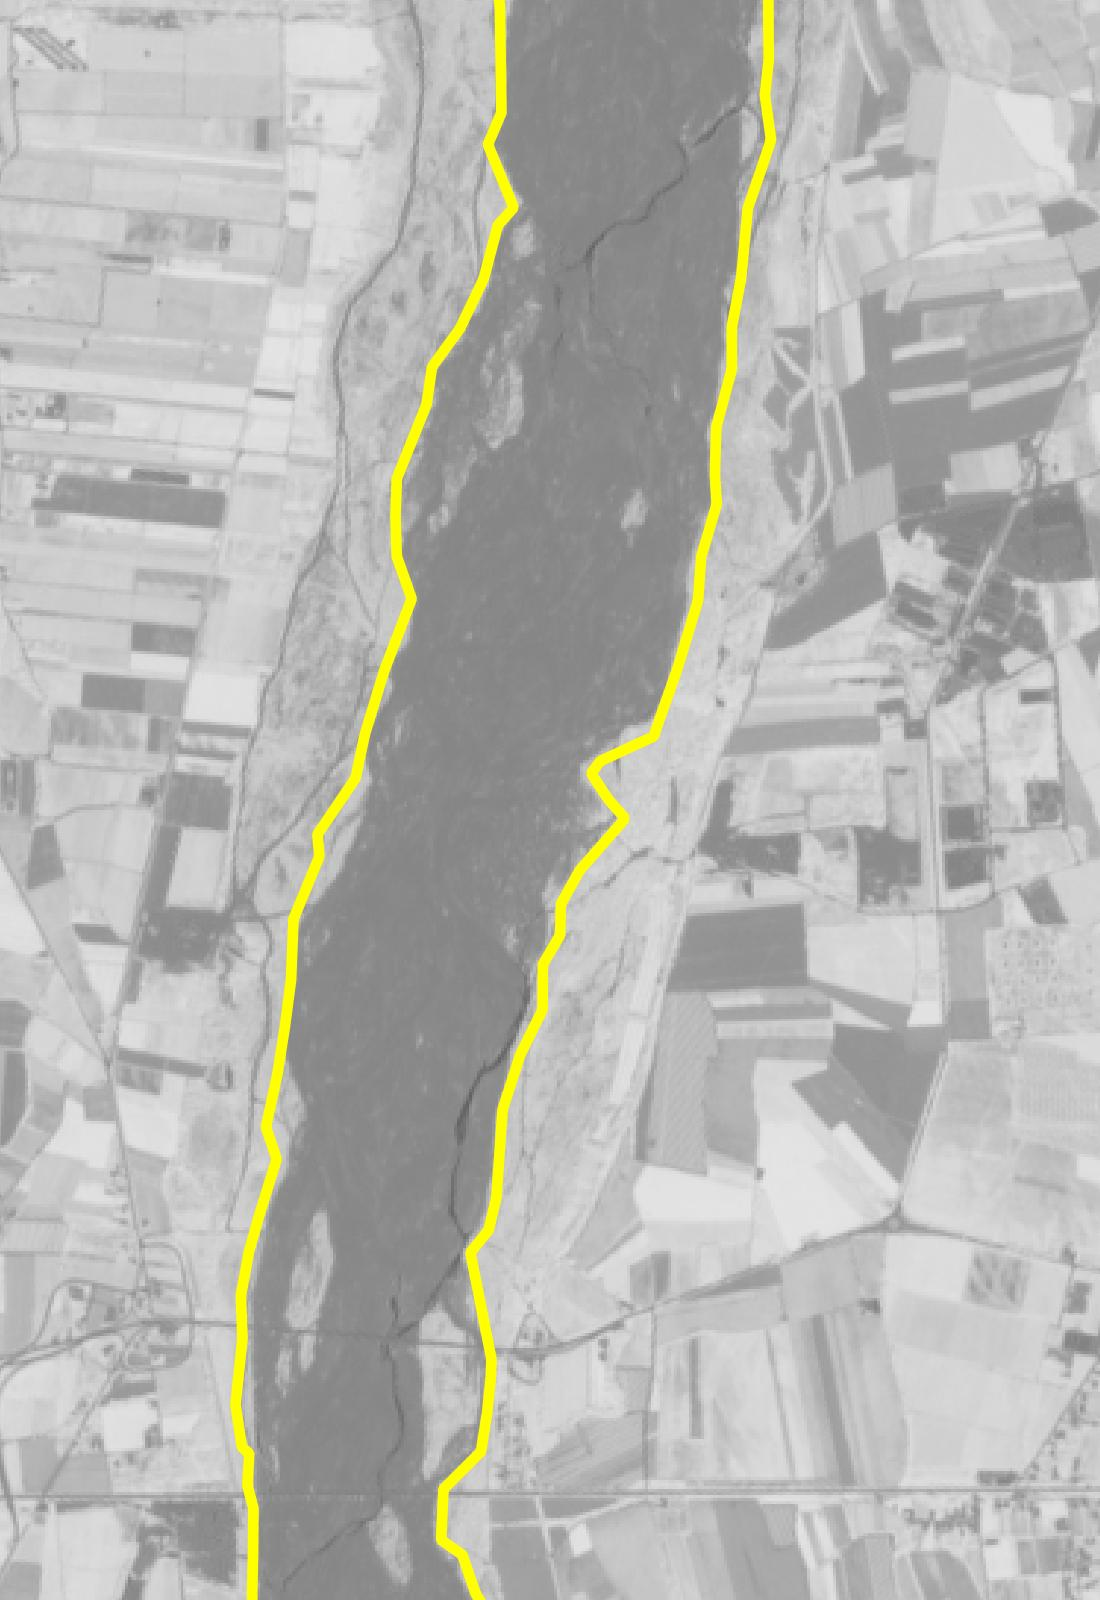
\includegraphics[width=\textwidth]{files/esempio_mask_2015_09_12.jpeg}
		\caption{\Se{} 2015-09-12.}
	\end{subfigure}
	\caption[definizione della maschera per limitare il dominio computazionale]
		{esempio in cui si vede come la maschera utilizzata per limitare il dominio computazionale (in giallo) sia il risultato dell'inviluppo degli alvei attivi che si sono modificati nel tempo; le immagini sono le mappe di NDVI.}
	\label{fig:esempio-maschera}
\end{figure}
%
%
\paragraph{NDVI} 
In questa area è stato calcolato il \emph{Normalized Difference Vegetation Index} (NDVI) grazie alle bande del \emph{Near Infrared} (NIR) e del \emph{Red} (R)
%
\begin{equation}
	%\notag
	NDVI = \frac{NIR - R}{NIR + R} \quad .
	\label{eq:ndvi}
\end{equation}
%
%
\paragraph{Aree campione}
\`{E} stata effettuata una digitalizzazione manuale di alcune aree campione per le immagini \AST{} del~2005-08-30 (\num{\sim 70}) e del~2012-08-01 (\num{\sim 100}), le immagini \Pl{} del~2014-10-31 (\num{\sim 40}) e del~2015-06-13 (\num{\sim 40}), l'immagine \Se{} del~2017-04-21 (\num{\sim 45}) e l'immagine \WV{} del 2018-06-15 (\num{\sim 55}) (\cref{fig:esempio-aree-campione}).
	Sono state selezionate immagini per ogni satellite poiché ciascuno è sensibile a bande leggermente diverse. 
	\\
	Queste aree campione sono state suddivise in tre classi: vegetazione, alveo attivo e canale.
	%
	\begin{figure}[ht]
		\centering
		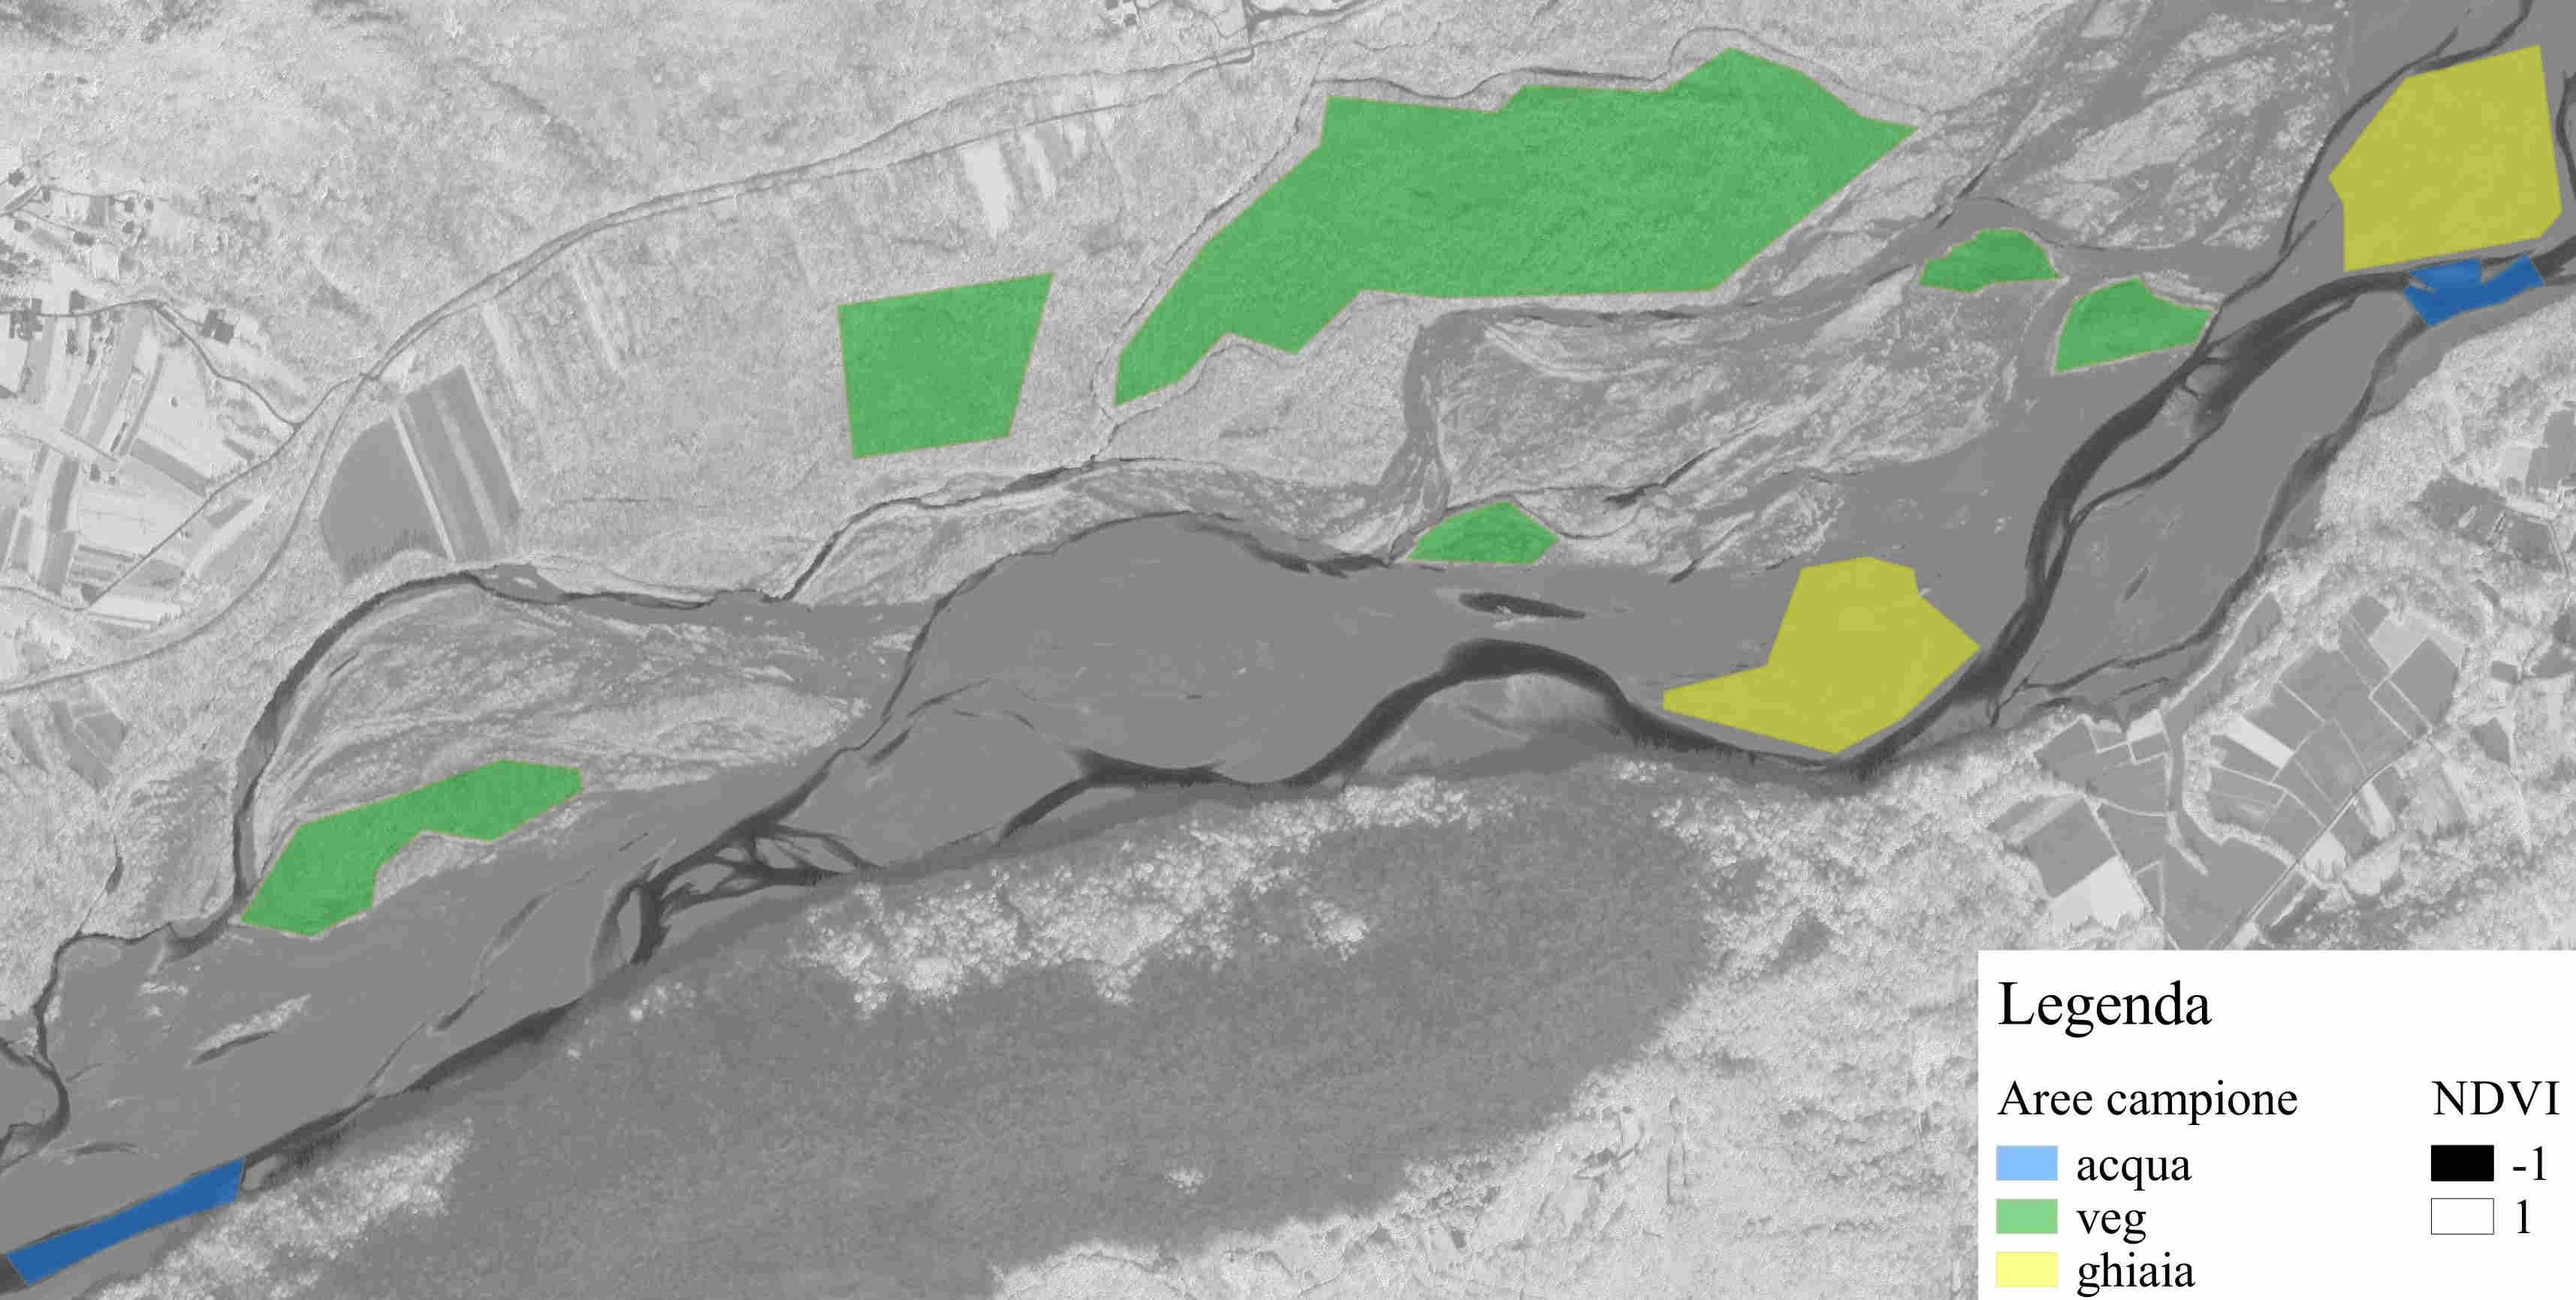
\includegraphics[width=\textwidth]{files/esempio_aree_campione_2014_10_31.jpeg}
		\caption[esempio di aree campione per calcolare la distribuzione dell'NDVI]{esempio di digitalizzazione di alcune aree campione per l'immagine \Pl{} del~2014-10-31 al fine di calcolare la distribuzione dell'NDVI caratteristica di tre diverse superfici; sullo sfondo la mappa dell'NDVI.}
		\label{fig:esempio-aree-campione}
	\end{figure}
	%
	%
\paragraph{Soglie NDVI}
Per ciascuna immagine si è osservata la distribuzione dell'NDVI in ogni classe tramite dei \emph{boxplot} (\cref{graph:percentili}): i \emph{boxplot} risultano essere nettamente separati gli uni dagli altri sia tra le scatole che tra i baffi; questo indica che le tre classi hanno distribuzioni di NDVI ben separate tra loro.
Ad esempio nella mappa dell'NDVI della \Pl{}~2014-10-31 il valore~\num{0.4} è sicuramente caratteristico della vegetazione e non dell'acqua; analogamente, valori superiori a~\num{0.2} sono certamente associati alla vegetazione, mentre valori inferiori sono associati a ghiaia o ad acqua.
% 
\begin{figure}[ht]
	\centering
	\begin{tikzpicture}
	\begin{groupplot}[
		group style = {
			group size = 2 by 3,
			ylabels at = edge left,
			x descriptions at = edge bottom,
			horizontal sep = 1.1cm,
			vertical sep = 0.1cm,
		},
		width = 0.45\textwidth,
		height = 0.45\textwidth,
		ylabel = NDVI,
		boxplot/draw direction = y,
		xtick = {1,2,3},
		xticklabels = {Veg., Alveo, Canale},
		ymax = 0.795,
		ymin = -0.50,
		grid = major,
	]
	\nextgroupplot % ASTER 2005-08-31
		\addplot+ [ % vegetazione
			teal, very thick,
			boxplot prepared = {
				lower whisker = 0.353656,
				lower quartile = 0.470411,
				median = 0.560063,
				upper quartile = 0.614701,
				upper whisker = 0.644957,
				},
        	]
        	coordinates {};
		\addplot+ [ % alveo attivo
			brown, very thick,
			boxplot prepared = {
				lower whisker = 0.077472,
				lower quartile = 0.091653,
				median = 0.122488,
				upper quartile = 0.149573,
				upper whisker = 0.171459,
				},
        	]
        	coordinates {};
		\addplot+ [ % canale
			cyan, very thick,
			boxplot prepared = {
				lower whisker = -0.477885,
				lower quartile = -0.362798,
				median = -0.269905,
				upper quartile = -0.058787,
				upper whisker = 0.072414,
				},
        	]
        	coordinates {};
        \node [fill = white, draw = black, anchor = north east] 
        	at (axis description cs: 1,1) {AST 2005-08-31};
	%------------------------------------------------------
	\nextgroupplot % ASTER 2012-08-01
		\addplot+ [ % vegetazione
			teal, very thick,
			boxplot prepared = {
				lower whisker = 0.341613,
				lower quartile = 0.444200,
				median = 0.586294,
				upper quartile = 0.672889,
				upper whisker = 0.709027,
				},
        	]
        	coordinates {};
		\addplot+ [ % alveo attivo
			brown, very thick,
			boxplot prepared = {
				lower whisker = 0.10506,
				lower quartile = 0.117969,
				median = 0.143631,
				upper quartile = 0.16549,
				upper whisker = 0.184871,
				},
        	]
        	coordinates {};
		\addplot+ [ % canale
			cyan, very thick,
			boxplot prepared = {
				lower whisker = -0.432201,
				lower quartile = -0.379825,
				median = -0.322239,
				upper quartile = -0.226459,
				upper whisker = -0.103914,
				},
        	]
        	coordinates {};
        \node [fill = white, draw = black, anchor = north east] 
        	at (axis description cs: 1,1) {AST 2012-08-01};
	%------------------------------------------------------
	\nextgroupplot % Pleiades 2014-10-31
		\addplot+ [ % vegetazione
			teal, very thick,
			boxplot prepared = {
				lower whisker = 0.286467,
				lower quartile = 0.350238,
				median = 0.415502,
				upper quartile = 0.483495,
				upper whisker = 0.549505,
				},
        	]
        	coordinates {};
		\addplot+ [ % alveo attivo
			brown, very thick,
			boxplot prepared = {
				lower whisker = 0.049796,
				lower quartile = 0.055794,
				median = 0.063049,
				upper quartile = 0.07173,
				upper whisker = 0.081427,
				},
        	]
        	coordinates {};
		\addplot+ [ % canale
			cyan, very thick,
			boxplot prepared = {
				lower whisker = -0.426415,
				lower quartile = -0.387978,
				median = -0.338308,
				upper quartile = -0.266515,
				upper whisker = -0.175373,
				},
        	]
        	coordinates {};
        \node [fill = white, draw = black, anchor = north east] 
        	at (axis description cs: 1,1) {PL 2014-10-31};
	%------------------------------------------------------
	\nextgroupplot % Pleiades 2015-08-13
		\addplot+ [ % vegetazione
			teal, very thick,
			boxplot prepared = {
				lower whisker = 0.415693,
				lower quartile = 0.5,
				median = 0.570359,
				upper quartile = 0.638507,
				upper whisker = 0.704044		
,
				},
        	]
        	coordinates {};
		\addplot+ [ % alveo attivo
			brown, very thick,
			boxplot prepared = {
				lower whisker = 0.075052,
				lower quartile = 0.080858,
				median = 0.087921,
				upper quartile = 0.096031,
				upper whisker = 0.106198,
				},
        	]
        	coordinates {};
		\addplot+ [ % canale
			cyan, very thick,
			boxplot prepared = {
				lower whisker = -0.262599,
				lower quartile = -0.244228,
				median = -0.214393,
				upper quartile = -0.176471,
				upper whisker = -0.132762,
				},
        	]
        	coordinates {};
        \node [fill = white, draw = black, anchor = north east] 
        	at (axis description cs: 1,1) {PL 2015-08-13};
	%------------------------------------------------------
	\nextgroupplot % Sentinel2 2017-04-21
		\addplot+ [ % vegetazione
			teal, very thick,
			boxplot prepared = {
				lower whisker = 0.163722,
				lower quartile = 0.241916,
				median = 0.374344,
				upper quartile = 0.548241,
				upper whisker = 0.672782,
				},
        	]
        	coordinates {};
		\addplot+ [ % alveo attivo
			brown, very thick,
			boxplot prepared = {
				lower whisker = 0.056176,
				lower quartile = 0.061278,
				median = 0.067681,
				upper quartile = 0.076396,
				upper whisker = 0.089304,
				},
        	]
        	coordinates {};
		\addplot+ [ % canale
			cyan, very thick,
			boxplot prepared = {
				lower whisker = -0.322237,
				lower quartile = -0.288822,
				median = -0.239533,
				upper quartile = -0.177094,
				upper whisker = -0.131119,
				},
        	]
        	coordinates {};
        \node [fill = white, draw = black, anchor = north east] 
        	at (axis description cs: 1,1) {S2 2017-04-21};
	%------------------------------------------------------
	\nextgroupplot % WorldView2 2018-06-15
		\addplot+ [ % vegetazione
			teal, very thick,
			boxplot prepared = {
				lower whisker = 0.569665,
				lower quartile = 0.657917,
				median = 0.719523,
				upper quartile = 0.759148,
				upper whisker = 0.791594,
				},
        	]
        	coordinates {};
		\addplot+ [ % alveo attivo
			brown, very thick,
			boxplot prepared = {
				lower whisker = 0.126214,
				lower quartile = 0.129661,
				median = 0.13373,
				upper quartile = 0.138542,
				upper whisker = 0.149326,
				},
        	]
        	coordinates {};
		\addplot+ [ % canale
			cyan, very thick,
			boxplot prepared = {
				lower whisker = -0.416974,
				lower quartile = -0.392405,
				median = -0.365385,
				upper quartile = -0.335135,
				upper whisker = -0.29979,
				},
        	]
        	coordinates {};
        \node [fill = white, draw = black, anchor = north east] 
        	at (axis description cs: 1,1) {WV2 2018-06-15};
	\end{groupplot}
\end{tikzpicture}

	\caption[\emph{boxplot} dell'NDVI nelle aree campione in quattro immagini satellitari]{\emph{boxplot} dell'NDVI nelle aree campione in quattro immagini satellitari per tre distinte superfici (di cui un esempio è riportato in \cref{fig:esempio-aree-campione}); i baffi indicano il $10_\mathrm{mo}$ e il $90_\mathrm{mo}$ percentile, gli estremi della scatola rappresentano il $25_\mathrm{mo}$ e il $75_\mathrm{mo}$ percentile, la linea nella scatola è la mediana.}
	\label{graph:percentili}
\end{figure}
%
\\
Da tali grafici sono state ottenute delle soglie di NDVI per classificare le immagini satellitari (\cref{tab:ndvi-soglia}); per l'immagine \WV{} la soglia che distingue vegetazione da alveo attivo è maggiore. 
Le soglie sono leggermente maggiori rispetto a quanto riportato in letteratura \squarecites{Bertoldi:2011-ASTER}{Henshaw:2013-LandSat} poiché in questo modo c'è una maggior corrispondenza con i dati utilizzati per validare il processo (riportati di seguito).
%
\begin{table}[ht]
	\centering
	\begin{tabular}{
		c 
		S[table-format=1.2]@{\,}
		c@{\,}
		c@{\,}
		c@{\,}
		S[table-format=1.2]
		S[table-format=1.2]@{\,}
		c@{\,}
		c@{\,}
		c@{\,}
		S[table-format=1.2]
		}
		\toprule
		&	\multicolumn{5}{c}{\textbf{Soglie AST PL S2}}	&	\multicolumn{5}{c}{\textbf{Soglie WV2}}	\\
		\midrule
		Vegetazione		&	0.25	&	$\leq$	&	NDVI	&			&		& 	0.30	&	$\leq$	&	NDVI	&			& 	\\
		Alveo attivo	&	0.00	&	$\leq$	&	NDVI	&	$<$		&	0.25	&	0.00	&	$\leq$	&	NDVI	&	$<$		&	0.30	\\
		Canale			&		&			&	NDVI	&	$<$		&	0.00	&		&			&	NDVI	&	$<$		&	0.00	\\
		\bottomrule
	\end{tabular}
	\caption[soglie NDVI]{soglie di NDVI per la classificazione delle immagini satellitari \AST{} (AST), \Pl{} (PL), \Se{} (S2) e \WV{} (WV2).}
	\label{tab:ndvi-soglia}
\end{table}
%
%
\paragraph{Isole e \emph{Floodplain}}
La maschera computazione individuata è unica per tutte le immagini in quanto è definita come l'inviluppo degli alvei attivi che si sono succeduti dal~2000 al~2018.
Il problema di questo approccio è che la copertura riparia delle isole non viene distinta da quella delle sponde.
Inoltre, a causa della bassa risoluzione delle immagini satellitari, i canali che separano isole molto prossime alla \emph{floodplain} dalle sponde stesse non vengono individuati e tali isole sembrano far completamente parte della \emph{floodplain}.
\\ 
Come soluzione è stata ideata una procedura semi-automatica che, con il supporto di Google Earth, divida la classe della vegetazione in \emph{floodplain} e isole. 
Tale procedura, sfruttando il fatto che le isole sono completamente circondate dalla ghiaia dell'alveo durante periodi di magra, classifica inizialmente la vegetazione più esterna come sponda;
poi corregge alcune celle della \emph{floodplain} convertendole in celle dell'alveo, separando nettamente le isole dalle sponde (\cref{fig:isola-divisa-floodplain}).
Le classi delle isole, delle sponde e delle celle corrette sono state aggiunte alla classificazione.
%
\begin{figure}
	\centering
	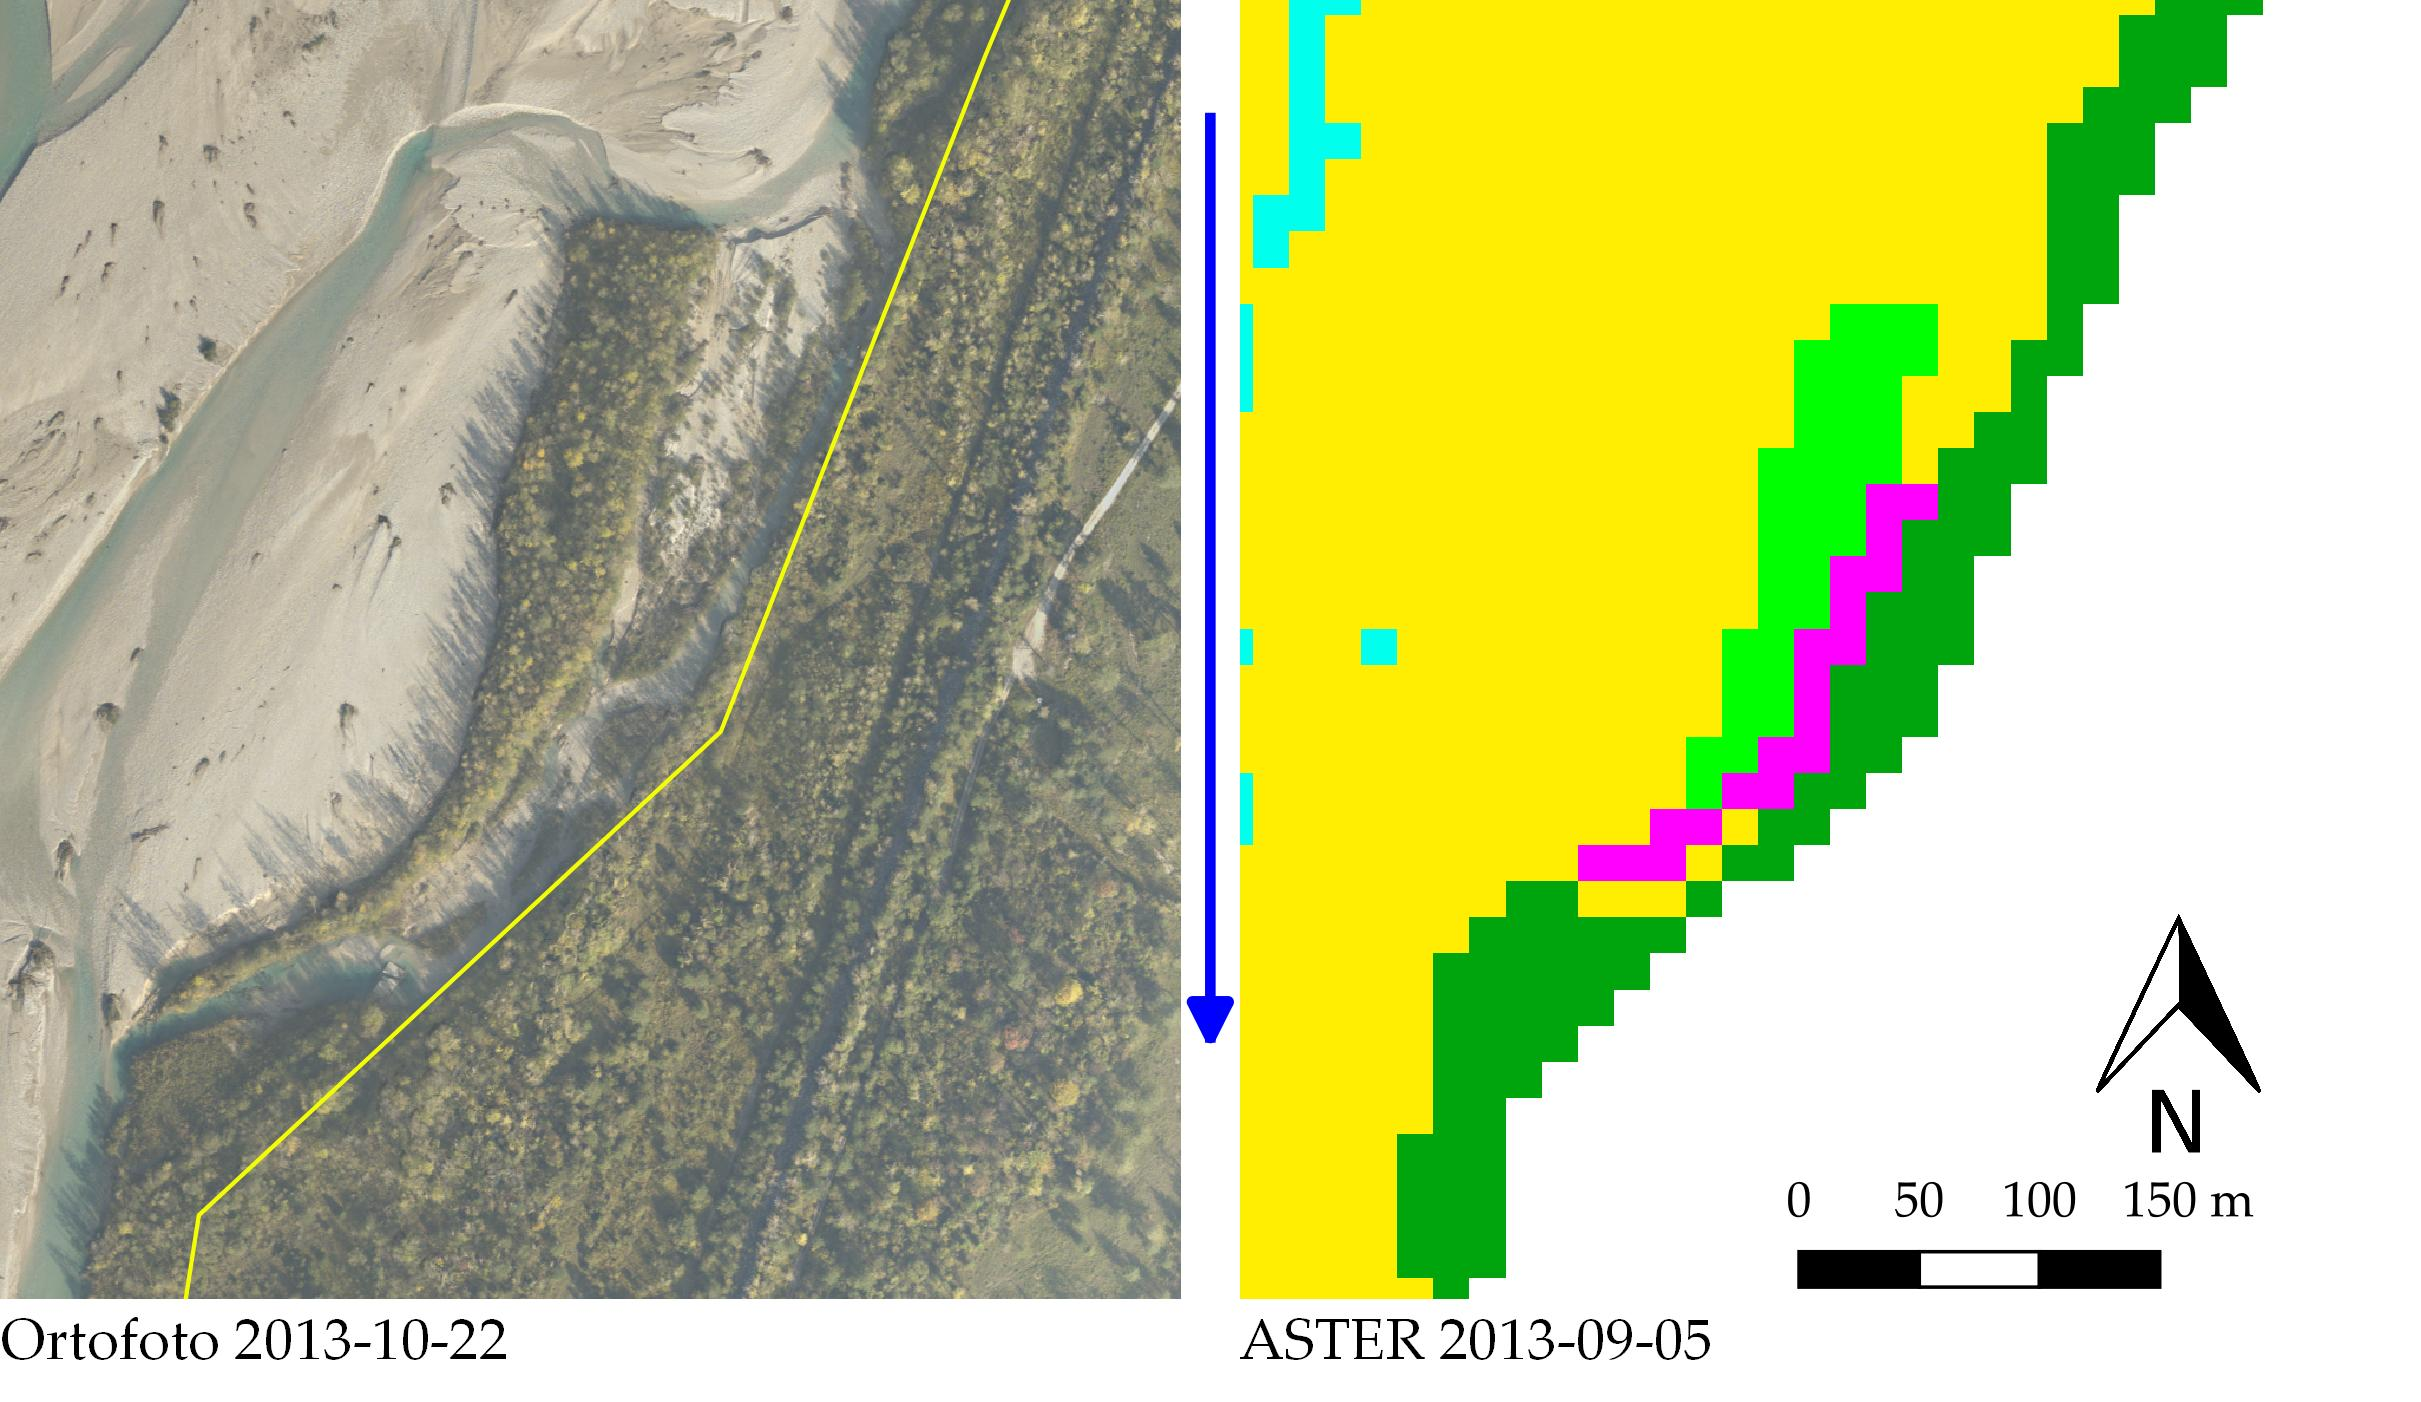
\includegraphics[width = \textwidth]{files/isola_divisa_floodplain.jpeg}
	\caption[esempio di correzione per dividere un'isola dalla sponda]{esempio di correzione per dividere un'isola dalla sponda; a sinistra si vede sull'ortofoto un'isola separata dalla \emph{floodplain} tramite un canale (in giallo è mostrato il limite della maschera computazionale); a destra si vede la stessa isola (verde chiaro) nell'immagine \AST{} temporalmente più vicina che è stata corretta (fucsia) per distinguerla dalla \emph{floodplain} (verde scuro); l'isola è circondata da ghiaia (giallo) e da acqua (azzurro).}
	\label{fig:isola-divisa-floodplain}
\end{figure}
%
%
%
\paragraph{Nuvole e nodata}
Alcune immagini presentano una lieve copertura nuvolosa che si estende nella maschera; queste zone sono state manualmente delimitate poiché presentano valori NDVI alterati.
\\
Altre immagini hanno un'estensione limitata rispetto alla maschera; questo porta ad avere aree prive di dati (\texttt{nodata}).
\\
Alla classificazione sono state aggiunte la classe delle nuvole e dei \texttt{nodata}.
%
%
\paragraph{Classificazione finale dei tratti}
La \cref{tab:class-tratti} mostra le classi in cui è stato classificato ognuno dei 23~tratti; la \cref{fig:class-is-fl} ne mostra un esempio.
%
\begin{table}[ht]
	\centering
	\begin{tabular}{
		c 
		c
		}
		\toprule
		\textbf{Macroclasse}	&	\textbf{Classe}	\\
		\midrule
		Vegetazione		&	Isola	\\
						&	Floodplain	\\
		\midrule
		Alveo attivo	&	Cella corretta	\\
						&	Ghiaia	\\
						&	Canale	\\
		\midrule
		Altro			&	Nuvola	\\
						&	Nodata	\\
		\bottomrule
	\end{tabular}
	\caption[classi della classificazione dei tratti]{classi della classificazione di ogni tratto all'interno della maschera computazionale.}
	\label{tab:class-tratti}
\end{table}
%
\begin{figure}[ht]
	\centering
	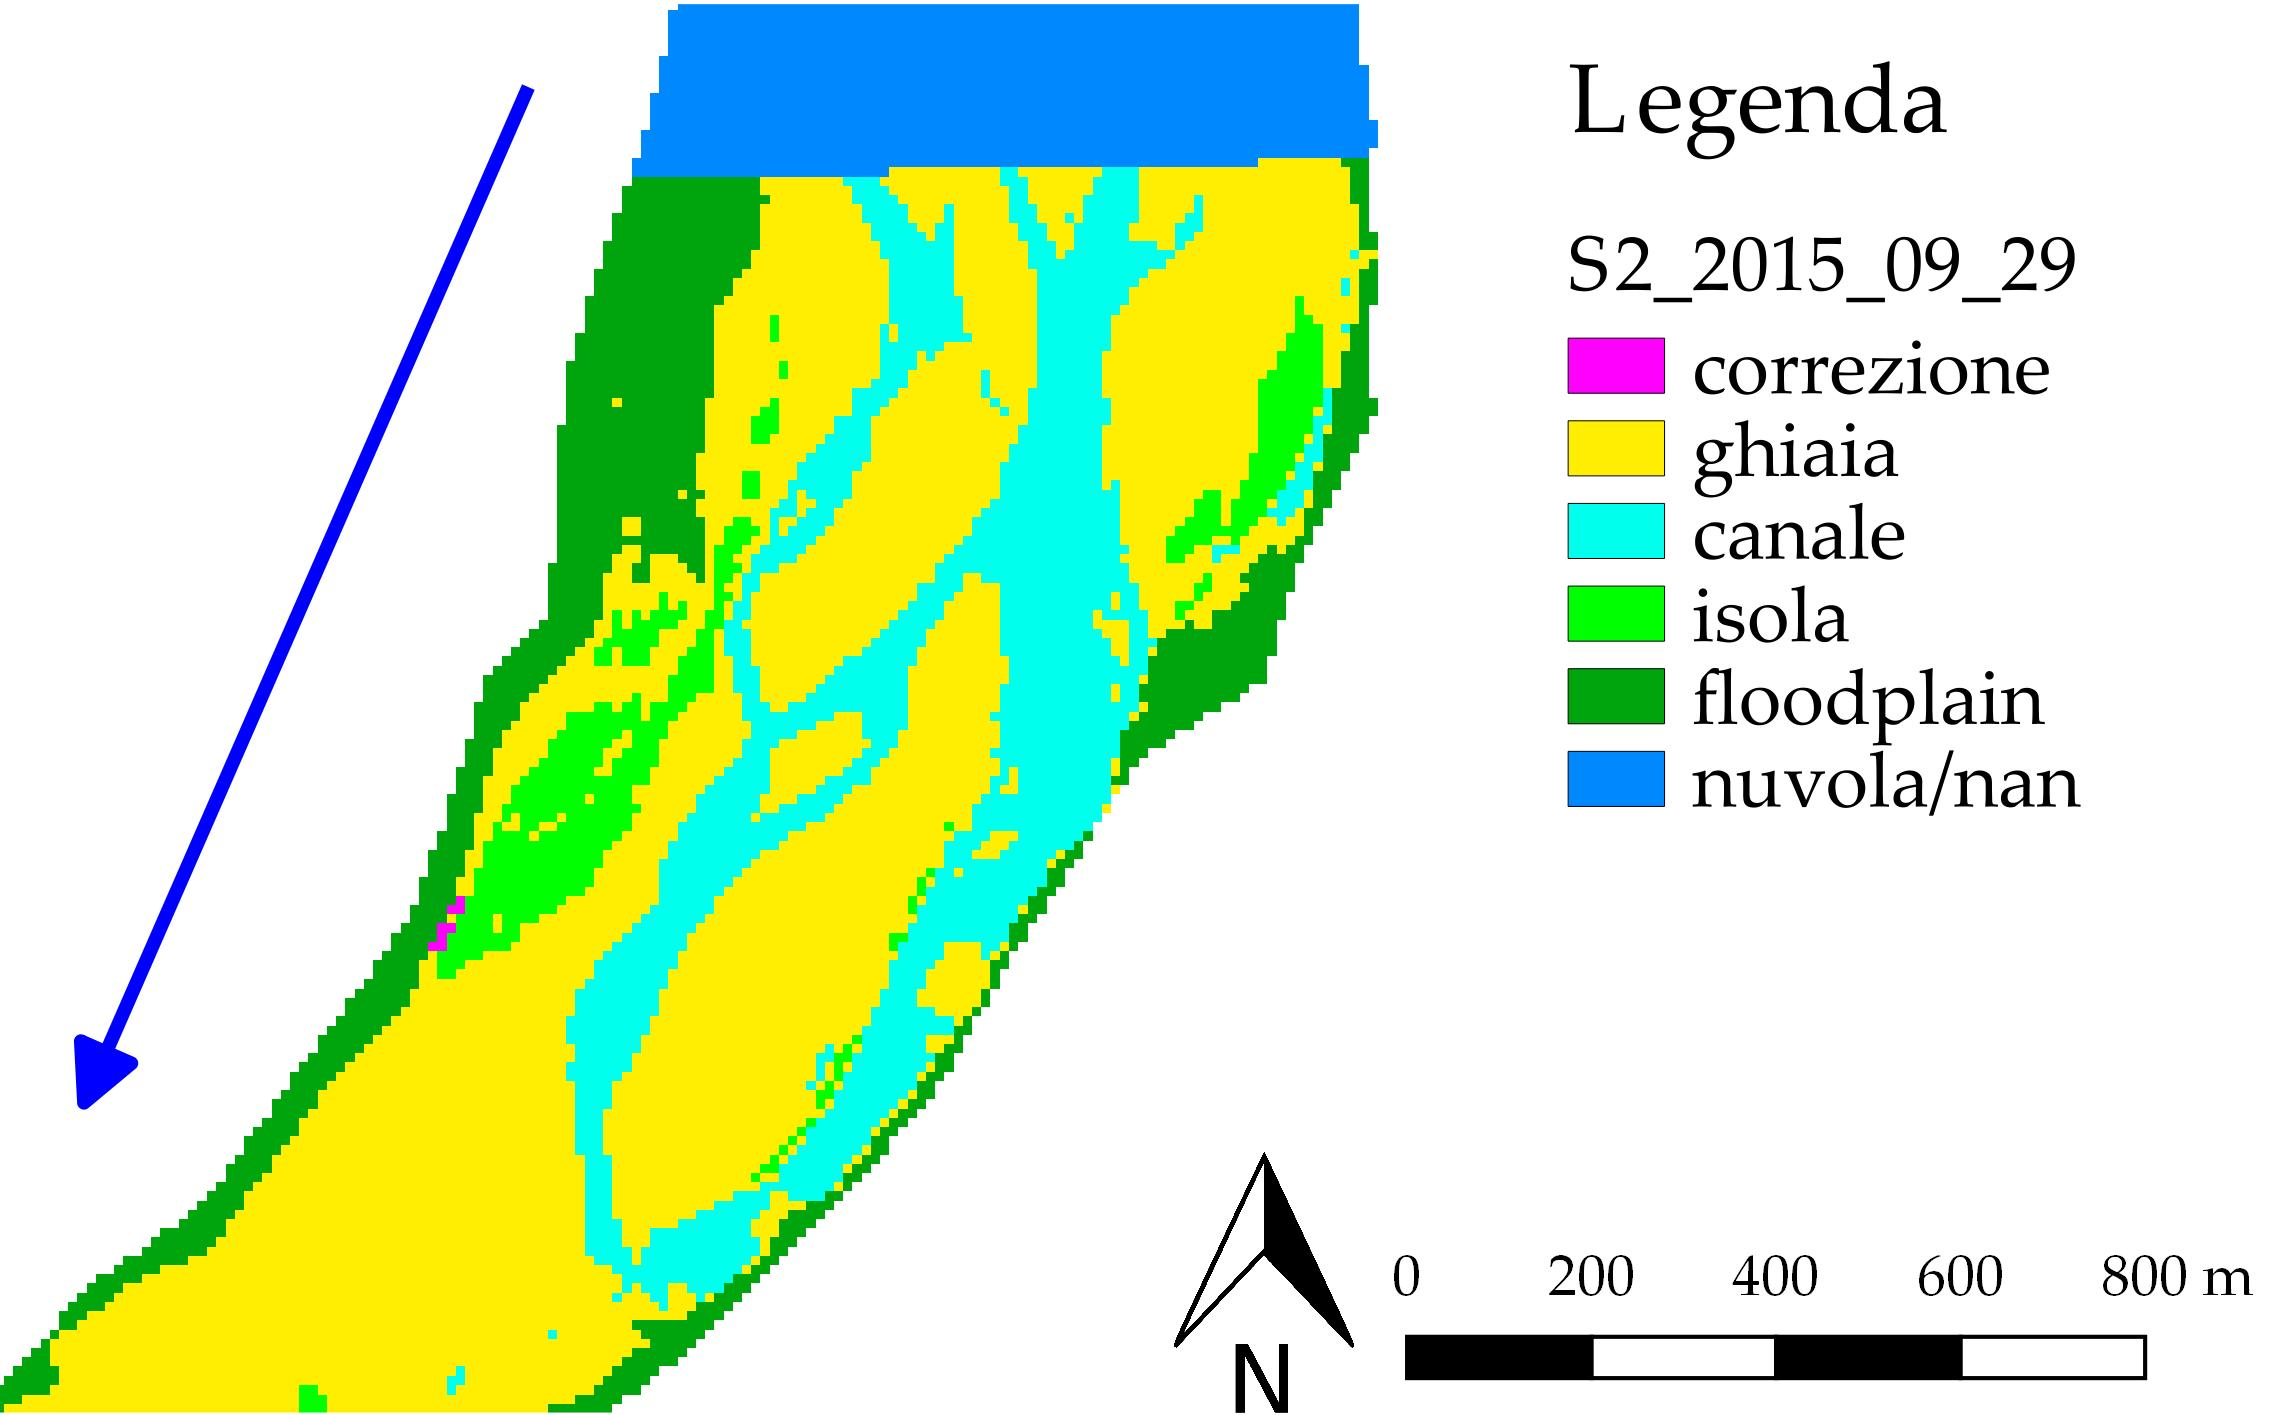
\includegraphics[width=\textwidth]{files/esempio_class_is_fl.jpeg}
	\caption[esempio della classificazione dei tratti]{esempio della classificazione dei tratti; le zone raffigurate sono rispettivamente a monte dell'isola di Cornino (in corrispondenza del monte Prat) e in corrispondenza della confluenza del Fella.}
	\label{fig:class-is-fl}
\end{figure}
%
%
%
\paragraph{Validazione}
Per controllare che la procedura restituisca risultati veritieri, si è confrontata la classificazione semi-automatica del 2011-10-02 con la classificazione eseguita manualmente da \squarecite{Surian:2015} nei tratti \numrange[range-phrase={$\div$}]{6}{12} (dal ponte autostradale di Braulins alla stretta di Pinzano).
Le mappe di classificazione del 2005-08-30, 2010-09-29, 2013-09-05 sono state confrontate con i CHM ricavati dai rilievi aerei LiDAR eseguiti nei corrispondenti anni su alcune porzioni dei tratti \numrange[range-phrase={$\div$}]{6}{12}.
Le immagini in \cref{fig:validazione-class-is-fl} mostrano alcuni confronti visuali tra classificazione semi-automatica e le immagini usate per la validazione.
Tra i rilievi LiDAR e le immagini \AST{} non hanno avuto luogo particolari eventi di piena, così come tra l'ortofoto del~2011 e la corrispondente immagine \AST{}.
%	
\begin{figure}
	\centering
	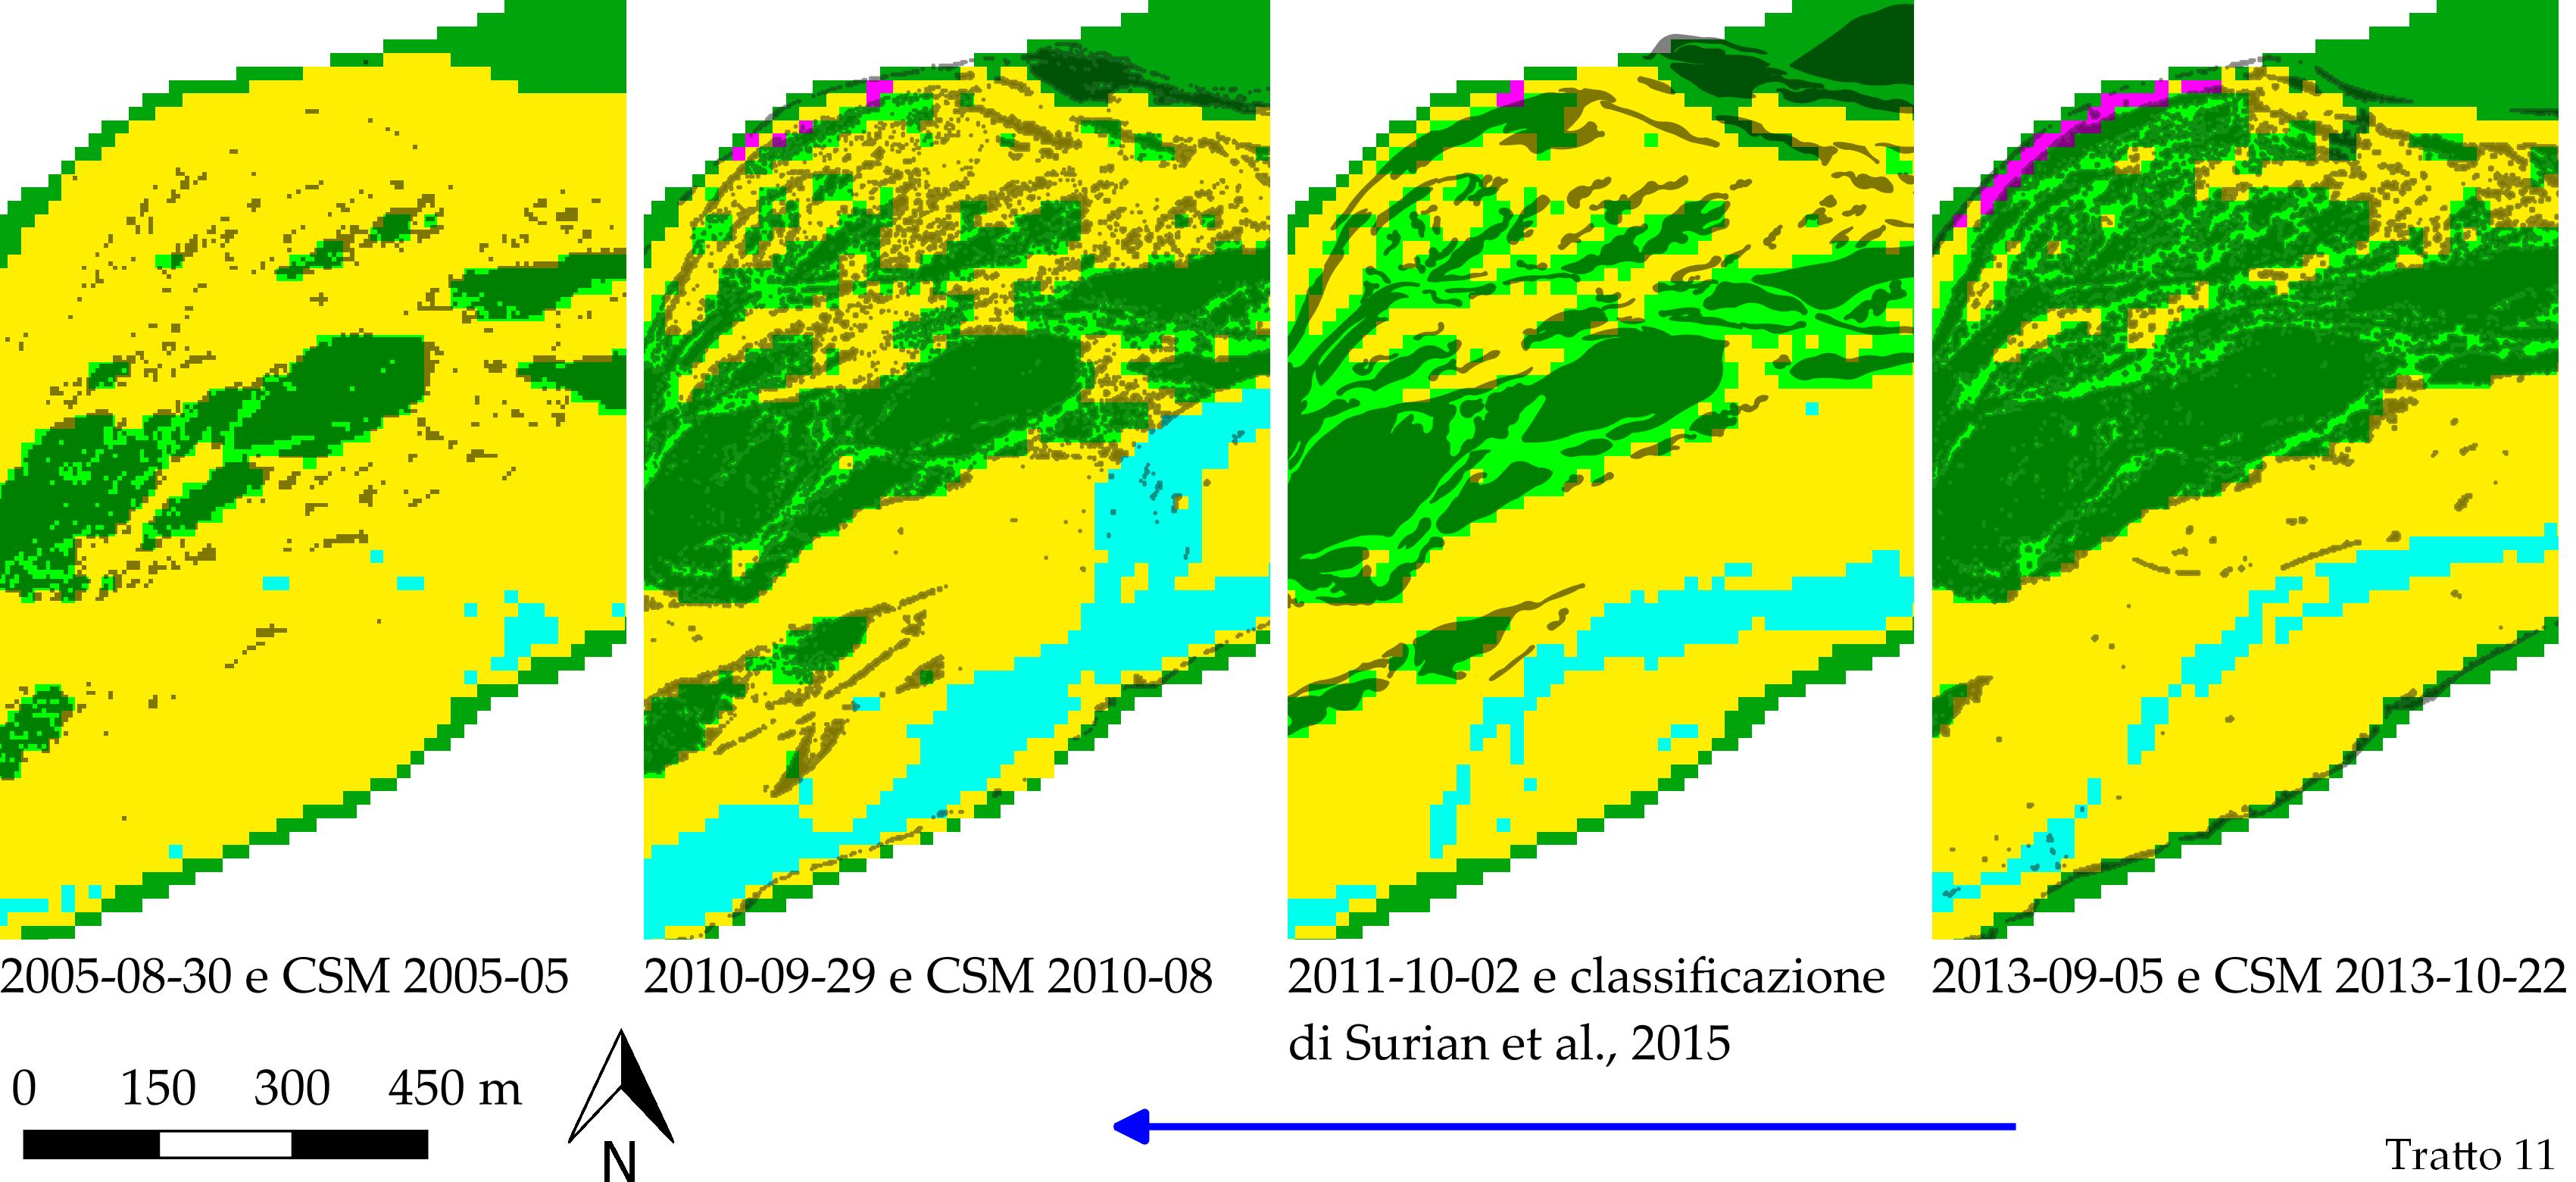
\includegraphics[width=\textwidth]{files/class_mia_vs_surian_chm.jpeg}
	\caption[validazione visuale della classificazione dell'alveo]{confronto tra le mappe di classificazione dell'alveo (sullo sfondo), i CHM ottenuti con rilievi aerei LiDAR e la classificazione manuale eseguita in \squarecite{Surian:2015} (in rosso semi-trasparente); le aree di sovrapposizione di rosso e verde chiaro indicano la corrispondenza tra la classificazione semi-automatica e i dati esterni; i colori indicano le isole (verde chiaro), le sponde (verde scuro), l'alveo (giallo), i canali (azzurro) e le celle corrette per distinguere le isole dalle sponde (fucsia).}
	\label{fig:validazione-class-is-fl}
\end{figure}
%
\begin{aenumerate}
	\item La classificazione manuale distingue la copertura arborea in tre tipi: alta, media e bassa.
	Le isole sono definite come le zone con alberi con un'area di \SI{\sim 100}{\m\tothe{2}}; nella presente tesi invece le isole sono definite come zone più o meno vegetate separate dalle sponde e circondate completamente da ghiaia e acqua, e questo porta a considerare come isole aree più ampie.
	\\
	La risoluzione minore delle immagini satellitari (principalmente a~\SI{10}{\m} o~\SI{15}{\m}) rispetto all'ortofoto (\SI{0.1}{\m}) permette di osservare macchie di vegetazione anziché i singoli alberi, delineando più nettamente il contorno delle isole maggiori; tuttavia le isole più piccole (con estensione minore di una cella) non sono individuate.
	\\
	Questa differenza nei metodi e nella definizione di isola porta ad una differenza del~\SI{-14}{\percent} dell'areale delle isole nella classificazione manuale rispetto a quella semi-automatica.
	%
	\item I CHM mostrano l'altezza della copertura arborea; dove questa altezza non è nulla, è presente vegetazione.
	La misura dell'altezza non si basa sul riconoscimento di un colore, come nella classificazione semi-automatica e manuale, ma sfrutta la riflessione di raggi laser da parte delle superfici, quali terreno e alberi; quindi i CHM costituiscono una fonte di validazione ben distinta dalla classificazione manuale.
	\\
	La somma delle aree con altezza della vegetazione non nulla nell'alveo costituisce l'area delle isole individuata per ogni CHM; rispetto alla classificazione semi-automatica, le differenze sono del \SIlist[list-separator = {, }, list-final-separator = { e }, retain-explicit-plus]{+22;+9;-3}{\percent} per i CHM del~2005, 2010 e~2013 rispettivamente.
\end{aenumerate}
%
Nel grafico in \cref{graph:validazione-class-is-fl} si vede l'areale delle isole nelle mappe di classificazione dell'alveo del~2005, 2010, 2011 e~2013 rispetto all'areale dalle mappe usate come validazione.
%
\begin{figure}
	\centering
	\tikzsetnextfilename{validazione_class_is_fl}
\begin{tikzpicture}
	\begin{axis}[
		width = 0.5\textwidth,
		height = 0.5\textwidth,
		xlabel = {Isole da NDVI \si{[\kilo\m\tothe{2}]}},
		ylabel = {Isole da CHM e class. manuale \si{[\kilo\m\tothe{2}]}},
		grid = major,
		]        
		\addplot[
			scatter,
			green!75!black,
			only marks,
			nodes near coords,
			%point meta = explicit symbolic,
			]
        	table [x expr = \thisrow{mie} / 1000000, y expr = \thisrow{CHM_Surian} / 1000000, point meta = \thisrow{anno}] {graphics/data/validazione_class_is_fl.txt};
        
		\addplot[
			blue,
			dashed,
			no markers,
			domain = 0.5:1.1,
			samples = 2,
			]
        	{x};
	\end{axis}
\end{tikzpicture}

	\caption[validazione della classificazione considerando le aree delle isole]{areale delle isole secondo la classificazione semi-automatica messa a confronto con quella secondo tre rilievi LiDAR e con una classificazione manuale \squarecite{Surian:2015}; la retta tratteggiata indica la situazione ideale in cui l'area delle isole ottenuta dalle immagini satellitari corrisponde a quella ottenuta con gli altri metodi; in ogni anno è stata considerata l'area delle isole nel tratto coperto dai CHM e dalla classificazione manuale.}
	\label{graph:validazione-class-is-fl}
\end{figure}
%
\\
C'è una certa differenza tra le isole individuate tramite la classificazione semi-automatica e quelle ottenute attraverso la classificazione manuale e i CHM, dovuta molto probabilmente ai diversi metodi di misura.
Da una parte, le mappe usate per la validazione mostrano isole con aree molto più piccole delle celle delle immagini satellitari e i CHM possono individuare come albero qualunque oggetto che si trovi sopra al terreno, come accumuli di legno o piloni della rete elettrica; dall'altra, tali mappe non classificano come isola le piccole aree ghiaiose o con vegetazione rada situate nel mezzo di isole ben sviluppate, come invece fa la classificazione semi-automatica.
\\
La differenza è stata calcolata solo per una piccola parte del tratto di studio poiché i dati di validazione non erano particolarmente estesi spazialmente.
In questa zona non sembra che la classificazione semi-automatica sovrastimi o sottostimi l'areale delle isole, ma che si collochi in una condizione intermedia.
\\
A fronte di quanto esposto, si ritiene che la classificazione eseguita sia sufficientemente valida.


\subsection{Larghezza}
Con i dati di classificazione dell'alveo è possibile calcolare la larghezza media~$B$ dell'alveo attivo, esprimibile semplicemente come il rapporto dell'area dell'alveo di ogni tratto (somma dell'alveo attivo e delle isole) rispetto alla sua lunghezza:
%
\begin{equation}
	\label{eq:larghezza-tratto}
	B = \frac{\text{Area alveo}}{Lunghezza} 
	\quad 
	\si{[\m]}
	\quad.
\end{equation}
% 
La lunghezza di un tratto è definita come la linea che,  seguendo la corrente, congiunge la sezione di monte a quella di valle; è unica per ogni tratto; il tratto più breve è l'8 (\SI{1260}{\m}) e il più lungo è il~17 (\SI{6340}{\m}).
In quanto le sezioni che definiscono ciascun tratto non cambiano nel tempo, anche la relativa lunghezza non cambia; l'area dell'alveo attivo, al contrario, può variare da un'immagine all'altra. 
%
%
\subsection{Potenza della corrente}
La potenza della corrente per unità di larghezza $\Omega$ in \si{[\watt\per\meter\tothe{2}]} è definita come:
%
\begin{equation}
	\label{eq:omega}
	\Omega = \frac{\rho \, g \, Q \, i_f}{B}
	\quad
	\si{[\watt\per\meter\tothe{2}]}
\end{equation}
%
dove:
%
\begin{itemize}
	\item $\rho$ è la densità dell'acqua, pari a \SI{1000}{\kilo\g\per\meter\tothe{3}};
	\item $g$ è l'accelerazione di gravità, pari a \SI{9.81}{\m\per\s\tothe{2}};
	\item $Q$ è la portata fluente nel canale misurata in \si{[\m\tothe{3}\per\s]};
	\item $i_f$ è la pendenza in \si{[\m\per\m]};
	\item $B$ è la larghezza del canale in \si{[\m]}.
\end{itemize}
%

Per ottenere la \emph{stream power} si è prima ottenuta la pendenza media di ogni tratto grazie al DEM del 2009 nella seguente maniera:
%
\begin{aenumerate}
	\item si è definita una coordinata curvilinea che segue il corso principale del fiume;
	\item sono state considerate le quote in tutti i punti sopra i quali scorre la coordinata curvilinea;
	\item è stata effettuata una regressione lineare tra la coordinata curvilinea e le quote raggruppando i tratti quattro a quattro (tranne per l'ultimo gruppo, formato dai tratti 21, 22 e 23);
	\item il coefficiente angolare della retta rappresenta la pendenza del gruppo di 4 tratti.
\end{aenumerate}
%
Il risultato è riportato nella \cref{tab:pendenza}.
%
\begin{table}
	\centering
	\begin{tabular}{
		S[list-separator={, }, list-final-separator={ e }]
		S[table-format=1.2]
	}
		\toprule
		\multicolumn{1}{c}{Tratti}	&	\multicolumn{1}{c}{Pendenza \si{[\percent]}}	\\
		\midrule
		\numlist{1;2;3;4}	&	0.52	\\
		\numlist{5;6;7;8}	&	0.48	\\
		\numlist{9;10;11;12}	&	0.23	\\
		\numlist{13;14;15;16}	&	0.40	\\
		\numlist{17;18;19;20}	&	0.31	\\
		\numlist{21;22;23}	&	0.25	\\
		\bottomrule
	\end{tabular}
	\caption[pendenze dei tratti]{pendenze dei tratti.}
	\label{tab:pendenza}
\end{table}
%
\\
In quanto modificazioni della pendenza avvengono in periodi di tempo di anni soprattutto in seguito ad eventi naturali e non di apporto o asporto di sedimenti, che non sono avvenuti in maniera diffusa ed intensa durante gli ultimi due decenni, si considera la pendenza ottenuta come rappresentativa e costante nel periodo di studio.
In più, questi valori sono in accordo con quanto presente in letteratura \squarecites{Arscott:2002-habitat-dynamics}{Gurnell:2006-omega}{Bertoldi:2010-d50}{Sitzia:2016-d50}.

Mentre la larghezza $B$ è nota per quasi ogni tratto in ogni immagine, la portata $Q$ non è nota.
Secondo quanto descritto nella sezione \ref{sec:descr-area-studio}, la percentuale di area di bacino drenante in ogni tratto può fornire un'informazione sulla portata fluente in quanto quest'ultima è approssimativamente proporzionale all'area drenante.
\\
Poiché i dati di livello alla stazione idrometrica di Villuzza rappresentano in maniera affidabile l'entità delle piene, si è deciso di riferire l'area drenante di ogni bacinoin ogni tratto rispetto a quella del tratto~12, posto immediatamente a monte del sensore idrometrico (si veda la \cref{fig:overview-sat} e la \cref{fig:23-tratti}).
In questo modo si suppone che, durante le piene, in ogni tratto scorra una portata che è proporzionale alla percentuale di bacino drenante rispetto al bacino sotteso alla stazione idrometrica; tale percentuale è minore dell’unità a monte della stazione, mentre è maggiore all’unità a valle della stazione.
Per definire l’area drenante in ogni tratto sono stati utilizzati i dati riguardo gli affluenti mostrati nell’introduzione.
\\
L'equazione~\eqref{eq:omega-finta} definisce formalmente la potenza della corrente fittizia utilizzata nel presente lavoro.
Per comodità e semplicità, la definizione e nomenclatura della potenza della corrente originale viene sostituita dalla potenza della corrente fittizia.
La nuova $\Omega$ si misura in \si{[\newton\per\m\tothe{4}]}.
%
\begin{equation}
	\label{eq:omega-finta}
	\Omega = \frac{A_\mathrm{tr}}{A_\mathrm{rif}} \, \frac{\rho \, g \, i_f}{B}	
	\quad
	\si{[\newton\per\m\tothe{4}]} 
\end{equation}
%
dove:
%
\begin{itemize}
	\item $A_\mathrm{tr}$ è l'area drenante di ogni tratto in \si{[\m\tothe{2}]};
	\item $A_\mathrm{rif}$ è l'area drenante del tratto~12, esattamente a monte del sensore idrometrico presso Villuzza, pari a \SI{2204}{\m\tothe{2}}.
\end{itemize}
%
Si noti che se durante una piena si avesse una misura affidabile di portata, moltiplicandola per questa $\Omega$ si otterrebbe la potenza della corrente precedentemente definita.
